192. \begin{figure}[ht!]
\center{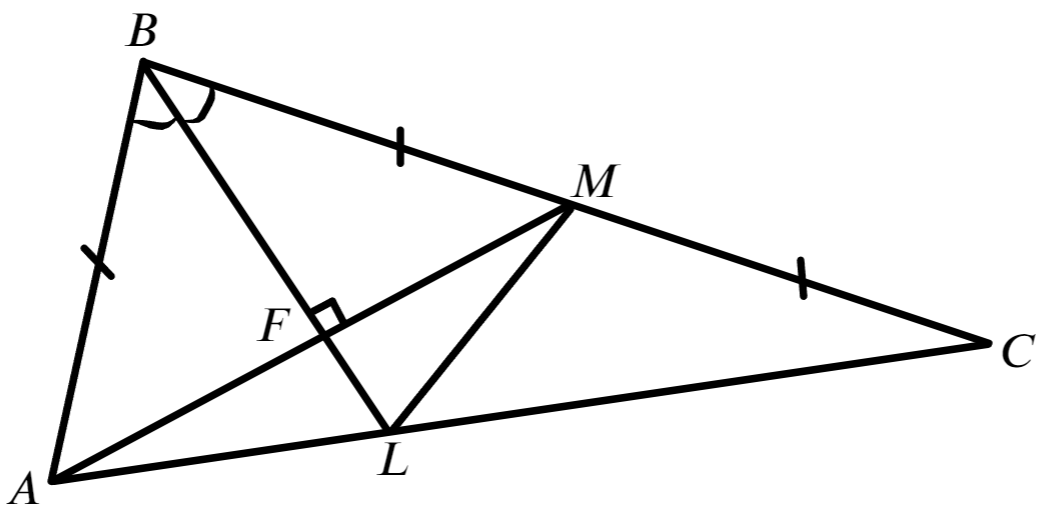
\includegraphics[scale=0.35]{g9-192.png}}
\end{figure}\\
В треугольнике $ABM$ биссектриса $BF$ совпала с высотой, значит он равнобедренный и $AB=BM,\ AF=FM.$ Тогда аналогично равнобедренным является и треугольник $AML$ (высота совпала с медианой), значит $S_{\Delta AFL}=S_{\Delta FML}=1.$ По свойству основания биссектрисы $\cfrac{AL}{LC}=\cfrac{AB}{BC}=\cfrac{1}{2}.$ Пусть $S_{\Delta ABF}=S_{\Delta BFM}=x.$ Так как площади треугольников с общей высотой относятся так же, как стороны, к которым она проведена, имеем соотношения
$x+x=1+1+S_{\Delta LMC},\ S_{\Delta LMC}=2x-2$ и $\cfrac{x+1}{x+1+2x-2}=\cfrac{1}{2},\ \cfrac{x+1}{3x-1}=\cfrac{1}{2},\ 2x+2=3x-1,\ x=3.$ Тогда $S_{\Delta ABC}=(3+3)\cdot2=12.$\\
